\documentclass[11pt,letterpaper,notumble]{leaflet}
\usepackage[T1]{fontenc}
\usepackage[utf8]{inputenc}
\usepackage{listingsutf8}
\usepackage[spanish]{babel}
\usepackage{microtype}
\usepackage{blindtext} 
\usepackage{biolinum} 
\renewcommand\rmdefault{\sfdefault}% Verwende serifenlose Schrift 
\usepackage{mwe}% Dummy Bilder 
\usepackage{graphicx}
\usepackage{verbatim}
\usepackage{xcolor}
	\definecolor{WildStrawberry}{rgb}{1.0, 0.26, 0.64}
	\definecolor{wildstrawberry}{rgb}{1.0, 0.26, 0.64}
	\definecolor{Mulberry}{rgb}{0.77, 0.29, 0.55}
	\definecolor{LimeGreen}{rgb}{0.2, 0.8, 0.2}
	\definecolor{LincolnGreen}{rgb}{0.11, 0.35, 0.02}
	\definecolor{blue}{rgb}{0.0, 0.0, 1.0}
	\definecolor{forestgreen(traditional)}{rgb}{0.0, 0.27, 0.13}
\usepackage[colorlinks,citecolor=blue,urlcolor=blue]{hyperref}


\AddToBackground{5}{\put(0,0){\textcolor{blue!5}{\rule{\paperwidth}{\paperheight}}}}%

\AddToBackground{5}{% Fondo de la página pequeña 1
	\put(\LenToUnit{0.05\paperwidth},\LenToUnit{0.875\paperheight}){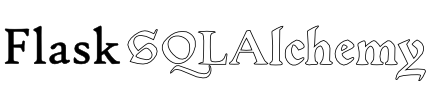
\includegraphics[width=\LenToUnit{0.90\paperwidth},height=\LenToUnit{0.1\paperheight}]{../img/flask-sqlalchemy-title.png}}
}

\title{Quik Reference} 
\author{Ferreira Juan David} 
\date{\today} % Experiment 1

\usepackage{float}
\begin{document}
    \mbox{}
    \thispagestyle{empty}% Keine Seitenzahlen 
    
    \newpage %page 2
    
    \makebox[\linewidth][l]{
    	\begin{minipage}{1.6\linewidth}
                	
            \begin{itemize}
            	\item No se encuentran elementos y \texttt{page} no es \texttt{1}.
            	
            	\item \texttt{page} es menor que \texttt{1} o \texttt{per\_page} es negativo.
            	
            	\item \texttt{page} o \texttt{per\_page} no son \texttt{ints}.
            \end{itemize}
            
            Cuando \texttt{error\_out} es \texttt{False}, \texttt{page} y el \texttt{per\_page} valor predeterminado es \texttt{1} y \texttt{20} respectivamente.
            
            Devuelve un objeto \texttt{Pagination}.
            
            \section{Sesiones}
            
            \texttt{class flask\_sqlalchemy.SignallingSession(db,autocommit=False, autoflush=True, **options)}
            
            La sesión de señalización es la sesión predeterminada que usa \texttt{Flask-SQLAlchemy}. Amplía el sistema de sesión predeterminado con selección de enlaces y seguimiento de modificaciones.
            
            Si desea utilizar una sesión diferente, puede anular la función \texttt{SQLAlchemy.create\_session()}.
            
            \textit{Nuevo en la versión 2.0}.
            
            \textit{Nuevo en la versión 2.1}: La liga se añadió opción, que permite que una sesión se unió a una transacción externa.
            
            \begin{description}
            	\item[\texttt{get\_bind(mapper=None, clause=None)}:] Devuelva el motor o la conexión para un modelo o tabla determinados, utilizando el \texttt{\_\_bind\_key\_\_} si está configurado.
            \end{description}
        
            \section{Utilities}
            
            \texttt{class flask\_sqlalchemy.Pagination(query, page, per\_page, total, items)}
            
            Del tipo \texttt{helper class} interna devuelta por \texttt{BaseQuery.paginate()}. También puede construirlo a partir de cualquier otro objeto de consulta \texttt{SQLAlchemy} si está trabajando con otras bibliotecas. Además, es posible pasar Ninguno como objeto de consulta, en cuyo caso \texttt{prev()} y \texttt{next()} dejarán de funcionar.
            \begin{description}
                \item[\texttt{has\_next}:]
                \texttt{True} si existe una página siguiente.
                
                \item[\texttt{has\_prev}:]
                \texttt{True} si existe una página anterior
                
                \item[\texttt{items=None}:] 
                los elementos de la página actual
                
                \item[\texttt{iter\_pages(left\_edge=2,left\_current=2,right\_current=5,right\_edge=2)}:] Repite los números de página en la paginación. Los cuatro parámetros controlan los umbrales cuántos números deben producirse desde los lados. Los números de página omitidos se representan como \texttt{None}. Así es como podría representar dicha paginación en las plantillas:
            \end{description}
        \end{minipage}
    
    }
    
    \newpage %page 3
    {\hspace{4.3cm}
    \makebox[\linewidth][l]{
    	\begin{minipage}{1.5\linewidth}
    		\lstset{inputencoding=utf8/latin1,
    			frame=lines,
    			label={lst:code_direct},
    			basicstyle=\footnotesize,
    			showstringspaces=false  
    		}
    		\lstinputlisting[language=html,firstline=1,lastline=15]{../python/08-API-Reference.html}
    		
    	    \begin{description}
    	    	
    	    	\item[\texttt{next(error\_out=False)}:]
    	    	Devuelve un objeto \texttt{Pagination} para la página siguiente.
    	    	
    	    	\item[\texttt{next\_num}:]
    	    	Número de la página siguiente.
    	    	
    	    	\item[\texttt{page= None}:] 
    	    	el número de página actual (\textit{1} indexado).
    	    	
    	    	\item[\texttt{pages}:]
    	    	El número total de páginas.
    	    	
    	    	\item[\texttt{per\_page= None}:] 
    	    	el número de elementos que se mostrarán en una página.
    	    	
    	    	\item[\texttt{prev(error\_out = False)}:]
    	    	Devuelve un objeto \texttt{Pagination} de la página anterior.
    	    	
    	    	\item[\texttt{prev\_num}:]
    	    	Número de la página anterior.
    	    	
    	    	\item[\texttt{query=None}:]
    	    	el objeto de consulta ilimitado que se utilizó para crear este objeto \texttt{Pagination}.
    	    	
    	    	\item[\texttt{total=None}:] 
    	    	el número total de elementos que coinciden con la consulta.
    	    	
    	    \end{description}
        
            \texttt{flask\_sqlalchemy.get\_debug\_queries()}
            
            En el modo de depuración, \texttt{Flask-SQLAlchemy} registrará todas las consultas \texttt{SQL} enviadas a la base de datos. Esta información está disponible hasta el final de la solicitud lo que permite asegurar fácilmente que el \texttt{SQL} generado es el esperado en errores o en pruebas unitarias. Si no desea habilitar el modo \texttt{DEBUG} para sus pruebas unitarias, también puede habilitar la grabación de consultas estableciendo la variable de configuración \texttt{'SQLALCHEMY\_RECORD\_QUERIES'} en \texttt{True}. Esto se habilita automáticamente si \texttt{Flask} está en modo de prueba.
            
            El valor devuelto será una lista de tuplas con nombre con los siguientes atributos: \texttt{statement}, \texttt{parameters}, \texttt{start\_time/end\_time}, \texttt{duration} y \texttt{context} (ver descripción en la documentación oficial).
    		
        \end{minipage}

    }}
    
    \newpage % page 4
    
    \mbox{}
    
    \newpage % page 5
    
    \maketitle
    
    \begin{abstract}
    	Si pensamos en utilizar una sola aplicación, podemos saltar este capítulo. Simplemente pasemos nuestra aplicación al constructor \texttt{SQLAlchemy} y estará listo. Sin embargo, si deseamos utilizar más de una aplicación o crear la aplicación dinámicamente en una función, debemos seguir leyendo.
    \end{abstract}

    \section{API Reference: Configuración}
    
    \begin{description}
    	\item[\texttt{get\_tables\_for\_bind(bind=None)}:] Devuelve una lista de todas las tablas relevantes para un enlace.
    	
    	\item[\texttt{init\_app(app)}:] Esta devolución de llamada se puede utilizar para inicializar una aplicación para su uso con esta configuración de base de datos. Nunca use una base de datos en el contexto de una aplicación que no se haya inicializado de esa manera o las conexiones se filtrarán.
    	
    	\item[\texttt{make\_connector(app=None, bind=None)}:]
    	Crea el conector para un estado y enlace determinados.
    	
    	\item[\texttt{metadata}:]
    	Los metadatos asociados con \texttt{db.Model}.
    \end{description}

    \thispagestyle{empty}
    
    \newpage
    
    \makebox[\linewidth][l]{
    	\begin{minipage}{2.2\linewidth}
            
            \begin{description}
            	
            	\item[\texttt{make\_declarative\_base(model, metadata=None)}:]
            	
            	Crea la base declarativa de la que heredarán todos los modelos.
            	
            	\textbf{Parámetros}
            	\begin{itemize}
            		\item \textbf{modelo}: clase de modelo base (o una tupla de clases base) a la que pasar \texttt{declarative\_base()}. O una clase devuelta \texttt{declarative\_base}, en cuyo caso no se crea una nueva clase base.
            		
            		\item \textbf{metadatos}: \texttt{MetaData} instancia para usar, o ninguna para usar el valor predeterminado de \texttt{SQLAlchemy}.
            	\end{itemize}
            	
            	\item[\texttt{reflect(bind = '\_\_all\_\_',app = None)}:]
            	Refleja tablas de la base de datos.
            	
            	\textit{Modificado en la versión 0.12}: se agregaron parámetros.
            	
            \end{description}
        
            \section{Models}
            
            \texttt{class flask\_sqlalchemy.Model}
            
            Clase base para el modelo base declarativo de \texttt{SQLAlchemy}.
            
            Para definir modelos, subclase \texttt{db.Model}, no esta clase. Para personalizar \texttt{db.Model}, subclase esto y pasarlo como \texttt{model\_class} a \texttt{SQLAlchemy}.
            
            \begin{description}
            	\item[\texttt{\_\_bind\_key\_\_}:] Opcionalmente declara el enlace que se utilizará. \texttt{None} se refiere al enlace predeterminado. Para obtener más información, consulte Varias bases de datos con enlaces.
            	
            	\item[\texttt{\_\_tablename\_\_}:]
            	El nombre de la tabla en la base de datos. Esto es requerido por \texttt{SQLAlchemy}; sin embargo, \texttt{Flask-SQLAlchemy} lo configurará automáticamente si un modelo tiene una clave primaria definida. Si \texttt{\_\_table\_\_} o \texttt{\_\_tablename\_\_} se establece explícitamente, se utilizará en su lugar.
            \end{description}
        
            \texttt{class flask\_sqlalchemy.BaseQuery(entities, session = None )} 
            Subclase \texttt{SQLAlchemy Query} con métodos convenientes para realizar consultas en una aplicación web.
            
            Este es el objeto \texttt{query} predeterminado que se usa para los modelos y se expone como \texttt{Query}. Reemplace la clase de consulta para un modelo individual subclasificando esto y estableciendo \texttt{query\_class}.
            
            \begin{description}
            	\item[\texttt{first\_or\_404(description=None)}:] Busca \texttt{first()} pero aborta con \texttt{404} si no se encuentra en lugar de regresar \texttt{None}.
            	\item[\texttt{get\_or\_404(ident, description=None)}:] Busca \texttt{get()} pero aborta con \texttt{404} si no se encuentra en lugar de regresar \texttt{None}.
            	\item[\texttt{paginate(page=None,per\_page=None,error\_out=True,max\_per\_page=None))}:] Devuelve artículos \texttt{per\_page} de la página \texttt{page}.
            	
            	Si \texttt{page} o \texttt{per\_page} son \texttt{None}, se recuperarán de la consulta de solicitud. Si \texttt{max\_per\_page} se especifica, \texttt{per\_page} se limitará a ese valor. Si no hay ninguna solicitud o no están en la consulta, se establecen de forma predeterminada en \texttt{1} y \texttt{20} respectivamente.
            	
            	Cuando \texttt{error\_out} es \texttt{True} (predeterminado), las siguientes reglas causarán una respuesta \texttt{404}:
            \end{description}
            
        \end{minipage}
    
    }

\end{document}